\subsection{\RU{Инструкции}\EN{Instructions}}
\label{sec:x86_instructions}

\RU{Инструкции, отмеченные как (M) обычно не генерируются компилятором: если вы видите её, очень может быть
это вручную написанный фрагмент кода, либо это т.н. compiler intrinsic}
\EN{Instructions marked as (M) are not usually generated by the compiler: if you see one of them, it is probably
a hand-written piece of assembly code, or a compiler intrinsic} (\myref{sec:compiler_intrinsic}).

% TODO ? обратные инструкции

\RU{Только наиболее используемые инструкции перечислены здесь}
\EN{Only the most frequently used instructions are listed here}.
\EN{You can read \myref{x86_manuals} for a full documentation.}%
\RU{Обращайтесь к \myref{x86_manuals} для полной документации.}

\RU{Нужно ли заучивать опкоды инструкций на память?}\EN{Do you have to know all instruction's opcodes by heart?}
\RU{Нет, только те, которые часто используются для модификации кода}\EN{No, only those
which are used for code patching} (\myref{x86_patching}).
\RU{Остальные запоминать нет смысла.}\EN{All the rest of the opcodes don't need to be memorized.}

\subsubsection{\RU{Префиксы}\EN{Prefixes}}

\myindex{x86!\Prefixes!LOCK}
\myindex{x86!\Prefixes!REP}
\myindex{x86!\Prefixes!REPE/REPNE}
\begin{description}
\label{x86_lock}
\item[LOCK] \RU{используется чтобы предоставить эксклюзивный доступ к памяти в многопроцессорной среде}
\EN{forces CPU to make exclusive access to the RAM in multiprocessor environment}.
\RU{Для упрощения, можно сказать, что когда исполняется инструкция с этим префиксом, остальные процессоры
в системе останавливаются}\EN{For the sake of simplification, it can be said that when an instruction
with this prefix is executed, all other CPUs in a multiprocessor system are stopped}.
\RU{Чаще все это используется для критических секций, семафоров, мьютексов}\EN{Most often
it is used for critical sections, semaphores, mutexes}.
\RU{Обычно используется с}\EN{Commonly used with} ADD, AND, BTR, BTS, CMPXCHG, OR, XADD, XOR.
\RU{Читайте больше о критических секциях}\EN{You can read more about critical sections here} (\myref{critical_sections}).

\item[REP] \RU{используется с инструкциями}\EN{is used with the} MOVSx \AndENRU STOSx\EN{ instructions}:
\RU{инструкция будет исполняться в цикле, счетчик расположен в регистре CX/ECX/RCX}
\EN{execute the instruction in a loop, the counter is located in the CX/ECX/RCX register}.
\RU{Для более детального описания, читайте больше об инструкциях}
\EN{For a detailed description, read more about the} MOVSx (\myref{REP_MOVSx}) 
\AndENRU STOSx (\myref{REP_STOSx})\EN{ instructions}.

\RU{Работа инструкций с префиксом REP зависит от флага DF, он задает направление}
\EN{The instructions prefixed by REP are sensitive to the DF flag, which is used to set the direction}.

\item[REPE/REPNE] (\ac{AKA} REPZ/REPNZ) \RU{используется с инструкциями}\EN{used with} CMPSx \AndENRU
SCASx\EN{ instructions}:
\RU{инструкция будет исполняться в цикле, счетчик расположен в регистре \TT{CX}/\TT{ECX}/\TT{RCX}}
\EN{execute the last instruction in a loop, the count is set in the \TT{CX}/\TT{ECX}/\TT{RCX} register}. 
\RU{Выполнение будет прервано если ZF будет 0 (REPE) либо если ZF будет 1 (REPNE)}
\EN{It terminates prematurely if ZF is 0 (REPE) or if ZF is 1 (REPNE)}.

\RU{Для более детального описания, читайте больше об инструкциях}
\EN{For a detailed description, you can read more about the} CMPSx (\myref{REPE_CMPSx}) 
\AndENRU SCASx (\myref{REPNE_SCASx})\EN{ instructions}.

\RU{Работа инструкций с префиксами REPE/REPNE зависит от флага DF, он задает направление}
\EN{Instructions prefixed by REPE/REPNE are sensitive to the DF flag, which is used to set the direction}.

\end{description}

\subsubsection{\RU{Наиболее часто используемые инструкции}\EN{Most frequently used instructions}}

\RU{Их можно заучить в первую очередь}\EN{These can be memorized in the first place}.

\begin{description}
% in order to keep them easily sorted...
\myindex{x86!\Instructions!ADC}
\myindex{x86!\Flags!CF}
  \item[ADC] (\IT{add with carry}) \RU{сложить два значения, \glslink{increment}{инкремент} 
  если выставлен флаг CF.
  ADC часто используется для складывания больших значений, например, складывания двух 64-битных
  значений в 32-битной среде используя две инструкции ADD и ADC, например:}
  \EN{add values, \gls{increment} the result if the CF flag is set.
  ADC is often used for the addition of large values, for example, 
  to add two 64-bit values in a 32-bit environment using two ADD and ADC instructions. For example:}

\EN{\lstinputlisting[style=customasmx86]{appendix/x86/instructions/ADC_example_EN.lst}}
\RU{\lstinputlisting[style=customasmx86]{appendix/x86/instructions/ADC_example_RU.lst}}

\RU{Еще один пример}\EN{One more example}: \myref{sec:64bit_in_32_env}.

\myindex{x86!\Instructions!ADD}
  \item[ADD] \RU{сложить два значения}\EN{add two values}

\myindex{x86!\Instructions!AND}
  \item[AND] \RU{логическое \q{И}}\EN{logical \q{and}}

\myindex{x86!\Instructions!CALL}
  \item[CALL] \RU{вызвать другую функцию}\EN{call another function}:\\
  \TT{PUSH address\_after\_CALL\_instruction; JMP label}

\myindex{x86!\Instructions!CMP}
\myindex{x86!\Instructions!SUB}
  \item[CMP] \RU{сравнение значений и установка флагов, то же что и \TT{SUB}, но только без записи результата}
  \EN{compare values and set flags, the same as \TT{SUB} but without writing the result}

\myindex{x86!\Instructions!DEC}
\myindex{x86!\Flags!CF}
  \item[DEC] \gls{decrement}.%
\RU{В отличие от других арифметических инструкций, \TT{DEC} не модифицирует флаг CF.}%
\EN{Unlike other arithmetic instructions, \TT{DEC} doesn't modify CF flag.}


\myindex{x86!\Instructions!IMUL} 
  \item[IMUL] \RU{умножение с учетом знаковых значений}\EN{signed multiply}
  \EN{\IMUL often used instead of \MUL, read more about it: \ref{IMUL_over_MUL}.}
% TODO translate


\myindex{x86!\Instructions!INC} 
\myindex{x86!\Flags!CF}
  \item[INC] \gls{increment}.%
\RU{В отличие от других арифметических инструкций, \TT{INC} не модифицирует флаг CF.}%
\EN{Unlike other arithmetic instructions, \TT{INC} doesn't modify CF flag.}

\myindex{x86!\Instructions!JCXZ}
\myindex{x86!\Instructions!JECXZ}
\myindex{x86!\Instructions!JRCXZ}
  \item[JCXZ, JECXZ, JRCXZ] (M) \RU{переход если CX/ECX/RCX=0}\EN{jump if CX/ECX/RCX=0}

\myindex{x86!\Instructions!JMP}
\item[JMP] \RU{перейти на другой адрес}\EN{jump to another address}.
\RU{Опкод имеет т.н.}\EN{The opcode has a} \gls{jump offset}.

\item[Jcc] (\RU{где}\EN{where} cc\EMDASH{}condition code)

\myindex{x86!\Instructions!JAE}
\myindex{x86!\Instructions!JA}
\myindex{x86!\Instructions!JBE}
\myindex{x86!\Instructions!JB}
\myindex{x86!\Instructions!JC}
\myindex{x86!\Instructions!JE}
\myindex{x86!\Instructions!JGE}
\myindex{x86!\Instructions!JG}
\myindex{x86!\Instructions!JLE}
\myindex{x86!\Instructions!JL}
\myindex{x86!\Instructions!JNAE}
\myindex{x86!\Instructions!JNA}
\myindex{x86!\Instructions!JNBE}
\myindex{x86!\Instructions!JNB}
\myindex{x86!\Instructions!JNC}
\myindex{x86!\Instructions!JNE}
\myindex{x86!\Instructions!JNGE}
\myindex{x86!\Instructions!JNG}
\myindex{x86!\Instructions!JNLE}
\myindex{x86!\Instructions!JNL}
\myindex{x86!\Instructions!JNO}
\myindex{x86!\Instructions!JNS}
\myindex{x86!\Instructions!JNZ}
\myindex{x86!\Instructions!JO}
\myindex{x86!\Instructions!JPO}
\myindex{x86!\Instructions!JP}
\myindex{x86!\Instructions!JS}
\myindex{x86!\Instructions!JZ}

\RU{Немало этих инструкций имеют синонимы (отмечены с AKA), это сделано для удобства}
\EN{A lot of these instructions have synonyms (denoted with AKA), this was done for convenience}.
\RU{Синонимичные инструкции транслируются в один и тот же опкод}
\EN{Synonymous instructions are translated into the same opcode}.
\RU{Опкод имеет т.н.}\EN{The opcode has a} \gls{jump offset}.

\label{Jcc}
\begin{description}
\item[JAE] \ac{AKA} JNC: \RU{переход если больше или равно (беззнаковый)}\EN{jump if above or equal (unsigned)}: CF=0
\EN{\item[JA] \ac{AKA} JNBE: jump if greater (unsigned): CF=0 and ZF=0}
\RU{\item[JA] \ac{AKA} JNBE: переход если больше (беззнаковый): CF=0 и ZF=0}
\EN{\item[JBE] jump if lesser or equal (unsigned): CF=1 or ZF=1}
\RU{\item[JBE] переход если меньше или равно (беззнаковый): CF=1 или ZF=1}
\item[JB] \ac{AKA} JC: \RU{переход если меньше (беззнаковый)}\EN{jump if below (unsigned)}: CF=1
\item[JC] \ac{AKA} JB: \RU{переход если CF=1}\EN{jump if CF=1}
\item[JE] \ac{AKA} JZ: \RU{переход если равно или ноль}\EN{jump if equal or zero}: ZF=1
\item[JGE] \RU{переход если больше или равно (знаковый)}\EN{jump if greater or equal (signed)}: SF=OF
\EN{\item[JG] jump if greater (signed): ZF=0 and SF=OF}
\RU{\item[JG] переход если больше (знаковый): ZF=0 и SF=OF}
\EN{\item[JLE] jump if lesser or equal (signed): ZF=1 or SF$\neq$OF}
\RU{\item[JLE] переход если меньше или равно (знаковый): ZF=1 или SF$\neq$OF}
\item[JL] \RU{переход если меньше (знаковый)}\EN{jump if lesser (signed)}: SF$\neq$OF
\item[JNAE] \ac{AKA} JC: \RU{переход если не больше или равно (беззнаковый)}\EN{jump if not above or equal (unsigned)} CF=1
\item[JNA] \RU{переход если не больше (беззнаковый)}\EN{jump if not above (unsigned)} CF=1 \AndENRU ZF=1
\item[JNBE] \RU{переход если не меньше или равно (беззнаковый)}\EN{jump if not below or equal (unsigned)}: CF=0 \AndENRU ZF=0
\item[JNB] \ac{AKA} JNC: \RU{переход если не меньше (беззнаковый)}\EN{jump if not below (unsigned)}: CF=0
\item[JNC] \ac{AKA} JAE: \RU{переход если CF=0, синонимично}\EN{jump CF=0 synonymous to} JNB.
\item[JNE] \ac{AKA} JNZ: \RU{переход если не равно или не ноль}\EN{jump if not equal or not zero}: ZF=0
\item[JNGE] \RU{переход если не больше или равно (знаковый)}\EN{jump if not greater or equal (signed)}: SF$\neq$OF
\EN{\item[JNG] jump if not greater (signed): ZF=1 or SF$\neq$OF}
\RU{\item[JNG] переход если не больше (знаковый): ZF=1 или SF$\neq$OF}
\item[JNLE] \RU{переход если не меньше (знаковый)}\EN{jump if not lesser (signed)}: ZF=0 \AndENRU SF=OF
\item[JNL] \RU{переход если не меньше (знаковый)}\EN{jump if not lesser (signed)}: SF=OF
\item[JNO] \RU{переход если не переполнение}\EN{jump if not overflow}: OF=0
\item[JNS] \RU{переход если флаг SF сброшен}\EN{jump if SF flag is cleared}
\item[JNZ] \ac{AKA} JNE: \RU{переход если не равно или не ноль}\EN{jump if not equal or not zero}: ZF=0
\item[JO] \RU{переход если переполнение}\EN{jump if overflow}: OF=1
\item[JPO] \RU{переход если сброшен флаг PF}\EN{jump if PF flag is cleared} (Jump Parity Odd)
\item[JP] \ac{AKA} \ac{JPE}: \RU{переход если выставлен флаг PF}\EN{jump if PF flag is set}
\item[JS] \RU{переход если выставлен флаг SF}\EN{jump if SF flag is set}
\item[JZ] \ac{AKA} JE: \RU{переход если равно или ноль}\EN{jump if equal or zero}: ZF=1
\end{description}


\myindex{x86!\Instructions!LAHF}
\myindex{x86!\Registers!AH}
  \item[LAHF] \RU{скопировать некоторые биты флагов в AH}\EN{copy some flag bits to AH}:

\begin{center}
\begin{bytefield}[endianness=big,bitwidth=0.03\linewidth]{8}
\bitheader{7,6,4,2,0} \\
\bitbox{1}{SF} & 
\bitbox{1}{ZF} & 
\bitbox{1}{} & 
\bitbox{1}{AF} & 
\bitbox{1}{} & 
\bitbox{1}{PF} & 
\bitbox{1}{} & 
\bitbox{1}{CF}
\end{bytefield}
\end{center}


\RU{Эта инструкция часто используется в коде работающем с \ac{FPU}.}
\EN{This instruction is often used in \ac{FPU}-related code.}


\myindex{x86!\Instructions!LEAVE}
\label{x86_ins:LEAVE}
\item[LEAVE] \RU{аналог команд \TT{MOV ESP, EBP} и \TT{POP EBP}\EMDASH{}
то есть возврат \glslink{stack pointer}{указателя стека} и регистра \EBP в первоначальное состояние.} 
\EN{equivalent of the \TT{MOV ESP, EBP} and \TT{POP EBP} instruction 
pair\EMDASH{}in other words, this instruction sets the \gls{stack pointer} (\ESP) back and restores 
the \EBP register to its initial state.}


\myindex{x86!\Instructions!LEA}
\item[LEA] (\IT{Load Effective Address}) \RU{сформировать адрес}\EN{form an address}

\label{sec:LEA}

\newcommand{\URLAM}{\href{http://go.yurichev.com/17109}{wikipedia}}

\RU{Это инструкция, которая задумывалась вовсе не для складывания 
и умножения чисел, 
а для формирования адреса например, из указателя на массив и прибавления индекса к нему
\footnote{См. также: \URLAM}.}
\EN{This instruction was intended not for summing values and multiplication 
but for forming an address, 
e.g., for calculating the address of an array element by adding the array address, element index, with 
multiplication of element size\footnote{See also: \URLAM}.}
\par
\RU{То есть, разница между \MOV и \LEA в том, что \MOV формирует адрес в памяти 
и загружает значение из памяти, либо записывает его туда, а \LEA только формирует адрес.}
\EN{So, the difference between \MOV and \LEA is that \MOV forms a memory address and loads a value
from memory or stores it there, but \LEA just forms an address.}
\par
\RU{Тем не менее, её можно использовать для любых других вычислений}
\EN{But nevertheless, it is can be used for any other calculations}.
\par
\RU{\LEA удобна тем, что производимые ею вычисления не модифицируют флаги \ac{CPU}. 
Это может быть очень важно для \ac{OOE} процессоров (чтобы было меньше зависимостей между данными).}
\EN{\LEA is convenient because the computations performed by it does not alter \ac{CPU} flags.
This may be very important for \ac{OOE} processors (to create less data dependencies).}

\RU{Помимо всего прочего, начиная минимум с Pentium, инструкция LEA исполняется за 1 такт.}%
\EN{Aside from this, starting at least at Pentium, LEA instruction is executed in 1 cycle.}

\begin{lstlisting}[style=customc]
int f(int a, int b)
{
	return a*8+b;
};
\end{lstlisting}

\begin{lstlisting}[caption=\Optimizing MSVC 2010,style=customasmx86]
_a$ = 8		; size = 4
_b$ = 12	; size = 4
_f	PROC
	mov	eax, DWORD PTR _b$[esp-4]
	mov	ecx, DWORD PTR _a$[esp-4]
	lea	eax, DWORD PTR [eax+ecx*8]
	ret	0
_f	ENDP
\end{lstlisting}

\myindex{Intel C++}
Intel C++ \RU{использует LEA даже больше}\EN{uses LEA even more}:

\begin{lstlisting}[style=customc]
int f1(int a)
{
	return a*13;
};
\end{lstlisting}

\begin{lstlisting}[caption=Intel C++ 2011,style=customasmx86]
_f1	PROC NEAR 
        mov       ecx, DWORD PTR [4+esp]      ; ecx = a
	lea       edx, DWORD PTR [ecx+ecx*8]  ; edx = a*9
	lea       eax, DWORD PTR [edx+ecx*4]  ; eax = a*9 + a*4 = a*13
        ret                                
\end{lstlisting}

\RU{Эти две инструкции вместо одной IMUL будут работать быстрее.}
\EN{These two instructions performs faster than one IMUL.}


\myindex{\CStandardLibrary!memcpy()}
\myindex{x86!\Instructions!MOVSB}
\myindex{x86!\Instructions!MOVSW}
\myindex{x86!\Instructions!MOVSD}
\myindex{x86!\Instructions!MOVSQ}
\item[MOVSB/MOVSW/MOVSD/MOVSQ] 
\RU{скопировать}\EN{copy} \RU{байт}\EN{byte}/
16-\RU{битное слово}\EN{bit word}/
32-\RU{битное слово}\EN{bit word}/
64-\RU{битное слово}\EN{bit word} \RU{на который указывает}\EN{from the address which is in} SI/ESI/RSI 
\RU{куда указывает}\EN{into the address which is in} DI/EDI/RDI.

\label{REP_MOVSx}
\myindex{x86!\Prefixes!REP}
\RU{Вместе с префиксом REP, инструкция исполняется в цикле, 
счетчик находится в регистре CX/ECX/RCX:}
\EN{Together with the REP prefix, it is to be repeated in a loop, 
the count is to be stored in the CX/ECX/RCX register:}
\RU{это работает как}\EN{it works like} memcpy() \RU{в Си}\EN{in C}.
\RU{Если размер блока известен компилятору на стадии компиляции,
memcpy() часто компилируется в короткий фрагмент кода использующий
REP MOVSx, иногда даже несколько инструкций}
\EN{If the block size is known to the compiler in the compile stage, 
memcpy() is often inlined into a short code fragment
using REP MOVSx, sometimes even as several instructions}.

\EN{The}\RU{Эквивалент} memcpy(EDI, ESI, 15)\EN{ equivalent is}:

\EN{\lstinputlisting[style=customasmx86]{appendix/x86/instructions/MOVSB_ex1_EN.asm}}
\RU{\lstinputlisting[style=customasmx86]{appendix/x86/instructions/MOVSB_ex1_RU.asm}}

(\RU{Должно быть, так быстрее чем копировать 15 байт используя просто одну REP MOVSB}
\EN{Supposedly, it works faster than copying 15 bytes using just one REP MOVSB}).


\myindex{x86!\Instructions!MOVSX}
  \item[MOVSX] \RU{загрузить с расширением знака}\EN{load with sign extension} \RU{см. также}\EN{see also}: (\myref{MOVSX})

\myindex{x86!\Instructions!MOVZX}
  \item[MOVZX] \RU{загрузить и очистить все остальные биты}\EN{load and clear all other bits} \RU{см. также}\EN{see also}: (\myref{movzx})

\myindex{x86!\Instructions!MOV}
\item[MOV] \RU{загрузить значение}\EN{load value}. \RU{эта инструкция была названа неудачно 
(данные не перемещаются, а копируются), 
что является результатом путаницы: 
в других архитектурах эта же инструкция называется \q{LOAD} и/или \q{STORE} или что-то в этом роде.}
\EN{this instruction name is misnomer, resulting in some confusion (data is not moved but copied), 
in other architectures the same instructions is usually named \q{LOAD} and/or \q{STORE} or something like that.}

\RU{Важно: если в 32-битном режиме при помощи MOV записывать младшую 16-байтную часть регистра,
то старшие 16 бит останутся такими же.}
\EN{One important thing: if you set the low 16-bit part of a 32-bit register in 32-bit mode, the high 16 bits
remains as they were.}
\RU{Но если в 64-битном режиме модифицировать 32-битную часть регистра, то старшие 32 бита обнуляются.}
\EN{But if you modify the low 32-bit part of the register in 64-bit mode, 
the high 32 bits of the register will be cleared.}

\RU{Вероятно, это сделано для упрощения портирования кода под x86-64.}
\EN{Supposedly, it was done to simplify porting code to x86-64.}

\ifdefined\BRAZILIAN
% TODO to be resynced:
Como curiosidade, vale ressaltar que \MOV é um nome equivocado para a instrução em ambos conjuntos de intruções do x86 e ARM, pois a informação não é de fato movida e sim copiada para o registrador ou variável de destino.
\fi % BRAZILIAN


\myindex{x86!\Instructions!MUL}
  \item[MUL] \RU{умножение с учетом беззнаковых значений}\EN{unsigned multiply}.
  \EN{\IMUL often used instead of \MUL, read more about it: \ref{IMUL_over_MUL}.}
% TODO translate


\myindex{x86!\Instructions!NEG}
  \item[NEG] \RU{смена знака}\EN{negation}: $op=-op$
\EN{Same as \TT{NOT op / ADD op, 1}.}
\RU{То же что и \TT{NOT op / ADD op, 1}.}


\myindex{x86!\Instructions!NOP}
\myindex{x86!\Instructions!XCHG}
  \item[NOP] \ac{NOP}. \RU{Её опкод 0x90, что на самом деле это холостая инструкция}
  \EN{Its opcode is 0x90, it is in fact the} 
  \TT{XCHG EAX,EAX}\EN{ idle instruction}.
  \RU{Это значит, что в x86 (как и во многих \ac{RISC}) нет отдельной \ac{NOP}-инструкции}
  \EN{This implies that x86 does not have a dedicated \ac{NOP} instruction (as in many \ac{RISC})}.
  \RU{В этой книге есть по крайней мере один листинг, где GDB отображает NOP как 16-битную инструкцию XCHG:}
  \EN{This book has at least one listing where GDB shows NOP as 16-bit XCHG instruction:}
  \myref{NOP_as_XCHG_example}.

  \RU{Еще примеры подобных операций}\EN{More examples of such operations}:
  (\myref{sec:npad}).

  \ac{NOP} \RU{может быть сгенерировать компилятором для выравнивания меток по 16-байтной границе}
  \EN{may be generated by the compiler for aligning labels on a 16-byte boundary}.
  \RU{Другое очень популярное использование}\EN{Another very popular usage of} \ac{NOP} 
  \RU{это вставка её вручную (патчинг) на месте какой-либо инструкции вроде условного перехода, чтобы
  запретить её исполнение}\EN{is to replace manually (patch) some instruction like a conditional jump
  to \ac{NOP} in order to disable its execution}.


\myindex{x86!\Instructions!NOT}
  \item[NOT] op1: $op1=\neg{}op1$. \RU{логическое \q{НЕ}}\EN{logical inversion}
  \RU{Важная особенность --- инструкция не меняет флаги.}
  \EN{Important feature---the instruction doesn't change flags.}

\myindex{x86!\Instructions!OR}
  \item[OR] \RU{логическое \q{ИЛИ}}\EN{logical \q{or}}

\myindex{x86!\Instructions!POP}
\EN{\item[POP] get a value from the stack: \TT{value=SS:[ESP]; ESP=ESP+4 (or 8)}}%
\RU{\item[POP] взять значение из стека: \TT{value=SS:[ESP]; ESP=ESP+4 (или 8)}}


\myindex{x86!\Instructions!PUSH}
\EN{\item[PUSH] push a value into the stack: \TT{ESP=ESP-4 (or 8); SS:[ESP]=value}}%
\RU{\item[PUSH] записать значение в стек: \TT{ESP=ESP-4 (или 8); SS:[ESP]=value}}


\myindex{x86!\Instructions!RET}
\myindex{MS-DOS}
\item[RET] \RU{возврат из процедуры}\EN{return from subroutine}: \TT{POP tmp; JMP tmp}.

\RU{В реальности}\EN{In fact}, RET 
\RU{это макрос ассемблера, в среде Windows и *NIX транслирующийся в}
\EN{is an assembly language macro, in Windows and *NIX environment it is translated into}
RETN (\q{return near}) 
\RU{ибо, во времена MS-DOS, где память адресовалась немного иначе}
\EN{or, in MS-DOS times, where the memory was addressed differently}
(\myref{8086_memory_model}), \RU{в}\EN{into} RETF (\q{return far}).

\RU{\TT{RET} может иметь операнд.}\EN{\TT{RET} can have an operand.}
\RU{Тогда его работа будет такой}\EN{Then it works like this}:\\
\TT{POP tmp; ADD ESP op1; JMP tmp}.
\TT{RET} \RU{с операндом обычно завершает функции с соглашением о вызовах \IT{stdcall}, см. также}
\EN{with an operand usually ends functions in the \IT{stdcall} calling convention, see also}: \myref{sec:stdcall}.


\myindex{x86!\Instructions!SAHF}
\myindex{x86!\Registers!AH}

  \item[SAHF] \RU{скопировать биты из AH в флаги CPU}\EN{copy bits from AH to CPU flags}:

\begin{center}
\begin{bytefield}[endianness=big,bitwidth=0.03\linewidth]{8}
\bitheader{7,6,4,2,0} \\
\bitbox{1}{SF} & 
\bitbox{1}{ZF} & 
\bitbox{1}{} & 
\bitbox{1}{AF} & 
\bitbox{1}{} & 
\bitbox{1}{PF} & 
\bitbox{1}{} & 
\bitbox{1}{CF}
\end{bytefield}
\end{center}


\RU{Эта инструкция часто используется в коде работающем с \ac{FPU}.}
\EN{This instruction is often used in \ac{FPU}-related code.}


\myindex{x86!\Instructions!SBB}
\myindex{x86!\Flags!CF}
  \item[SBB] (\IT{subtraction with borrow}) 
  \RU{вычесть одно значение из другого, \glslink{decrement}{декремент} результата если флаг CF выставлен.
  SBB часто используется для вычитания больших значений, например, для вычитания двух 64-битных
  значений в 32-битной среде используя инструкции SUB и SBB, например:}
  \EN{subtract values, \gls{decrement} the result if the CF flag is set.
  SBB is often used for subtraction of large values, for example,
  to subtract two 64-bit values in 32-bit environment using two SUB and SBB instructions. For example:}

\EN{\lstinputlisting[style=customasmx86]{appendix/x86/instructions/SBB_example_EN.lst}}
\RU{\lstinputlisting[style=customasmx86]{appendix/x86/instructions/SBB_example_RU.lst}}

\RU{Еще один пример}\EN{One more example}: \myref{sec:64bit_in_32_env}.

\myindex{\CStandardLibrary!strlen()}
\myindex{\CStandardLibrary!memchr()}
\myindex{x86!\Instructions!SCASB}
\myindex{x86!\Instructions!SCASW}
\myindex{x86!\Instructions!SCASD}
\myindex{x86!\Instructions!SCASQ}
\item[SCASB/SCASW/SCASD/SCASQ] (M) \RU{сравнить}\EN{compare} \RU{байт}\EN{byte}/
16-\RU{битное слово}\EN{bit word}/
32-\RU{битное слово}\EN{bit word}/
64-\RU{битное слово,}\EN{bit word} \RU{записанное в}\EN{that's stored in}
AX/EAX/RAX \RU{со значением, адрес которого находится
в}\EN{with a variable whose address is in} DI/EDI/RDI.
\RU{Выставить флаги так же, как это делает \CMP}\EN{Set flags as \CMP does}.

\label{REPNE_SCASx}
\myindex{x86!\Prefixes!REPNE}
\RU{Эта инструкция часто используется с префиксом REPNE: продолжать сканировать буфер до тех
пор, пока не встретится специальное значение, записанное в AX/EAX/RAX}
\EN{This instruction is often used with the REPNE prefix: continue to scan the buffer until a special value
stored in AX/EAX/RAX is found}.
\RU{Отсюда \q{NE} в REPNE: продолжать сканирование если сравниваемые значения не равны и остановиться
если равны}
\EN{Hence \q{NE} in REPNE: continue to scan while the compared values are not equal and stop when equal}.

\RU{Она часто используется как стандартная функция Си strlen(), для определения длины \ac{ASCIIZ}-строки}
\EN{It is often used like the strlen() C standard function, to determine an \ac{ASCIIZ} string's length}:

\RU{Пример}\EN{Example}:

\EN{\lstinputlisting[style=customasmx86]{appendix/x86/instructions/SCASB_ex1_EN.asm}}
\RU{\lstinputlisting[style=customasmx86]{appendix/x86/instructions/SCASB_ex1_RU.asm}}

\RU{Если использовать другое значение AX/EAX/RAX, функция будет работать как стандартная функция Си memchr(),
т.е. для поиска определенного байта.}
\EN{If we use a different AX/EAX/RAX value, the function acts like the memchr() standard C function, i.e.,
it finds a specific byte.}


\myindex{x86!\Instructions!SHL}
\myindex{x86!\Instructions!SHR}
  \item[SHL] \RU{сдвинуть значение влево}\EN{shift value left}
  \item[SHR] \RU{сдвинуть значение вправо}\EN{shift value right}:

\begin{center}
	\begin{tikzpicture}[scale=0.7, every node/.style={scale=0.7}]
	\edef\bitsize{1cm}
	\tikzstyle{byte}=[draw,minimum size=\bitsize]	
	\tikzstyle{every path}=[thick]

	\node [draw,rectangle,minimum size=\bitsize] (a1) {7};
	\node [draw,rectangle,minimum size=\bitsize] (a2) [right of=a1] {6};
	\node [draw,rectangle,minimum size=\bitsize] (a3) [right of=a2] {5};
	\node [draw,rectangle,minimum size=\bitsize] (a4) [right of=a3] {4};
	\node [draw,rectangle,minimum size=\bitsize] (a5) [right of=a4] {3};
	\node [draw,rectangle,minimum size=\bitsize] (a6) [right of=a5] {2};
	\node [draw,rectangle,minimum size=\bitsize] (a7) [right of=a6] {1};
	\node [draw,rectangle,minimum size=\bitsize] (a8) [right of=a7] {0};

	\node (empty) [below of=a1] {};

	\node [draw,rectangle,minimum size=\bitsize] (b1) [below of=empty] {7};
	\node [draw,rectangle,minimum size=\bitsize] (b2) [right of=b1] {6};
	\node [draw,rectangle,minimum size=\bitsize] (b3) [right of=b2] {5};
	\node [draw,rectangle,minimum size=\bitsize] (b4) [right of=b3] {4};
	\node [draw,rectangle,minimum size=\bitsize] (b5) [right of=b4] {3};
	\node [draw,rectangle,minimum size=\bitsize] (b6) [right of=b5] {2};
	\node [draw,rectangle,minimum size=\bitsize] (b7) [right of=b6] {1};
	\node [draw,rectangle,minimum size=\bitsize] (b8) [right of=b7] {0};
	
	\node [shape=rectangle,draw,minimum size=\bitsize] (d) [left=of b1] {CF};
	\node [shape=rectangle,draw,minimum size=\bitsize] (c) [right=of b8] {0};
	
	\draw [->] (c.west) -- (b8.east);

	\draw [->] (a2.south) -- (b1.north);
	\draw [->] (a3.south) -- (b2.north);
	\draw [->] (a4.south) -- (b3.north);
	\draw [->] (a5.south) -- (b4.north);
	\draw [->] (a6.south) -- (b5.north);
	\draw [->] (a7.south) -- (b6.north);
	\draw [->] (a8.south) -- (b7.north);
	
	\draw [->] (a1.south) -- (d.north);

	\end{tikzpicture}
\end{center}

\begin{center}
	\begin{tikzpicture}[scale=0.7, every node/.style={scale=0.7}]
	\edef\bitsize{1cm}
	\tikzstyle{byte}=[draw,minimum size=\bitsize]	
	\tikzstyle{every path}=[thick]

	\node [draw,rectangle,minimum size=\bitsize] (a1) {7};
	\node [draw,rectangle,minimum size=\bitsize] (a2) [right of=a1] {6};
	\node [draw,rectangle,minimum size=\bitsize] (a3) [right of=a2] {5};
	\node [draw,rectangle,minimum size=\bitsize] (a4) [right of=a3] {4};
	\node [draw,rectangle,minimum size=\bitsize] (a5) [right of=a4] {3};
	\node [draw,rectangle,minimum size=\bitsize] (a6) [right of=a5] {2};
	\node [draw,rectangle,minimum size=\bitsize] (a7) [right of=a6] {1};
	\node [draw,rectangle,minimum size=\bitsize] (a8) [right of=a7] {0};

	\node (empty) [below of=a1] {};

	\node [draw,rectangle,minimum size=\bitsize] (b1) [below of=empty] {7};
	\node [draw,rectangle,minimum size=\bitsize] (b2) [right of=b1] {6};
	\node [draw,rectangle,minimum size=\bitsize] (b3) [right of=b2] {5};
	\node [draw,rectangle,minimum size=\bitsize] (b4) [right of=b3] {4};
	\node [draw,rectangle,minimum size=\bitsize] (b5) [right of=b4] {3};
	\node [draw,rectangle,minimum size=\bitsize] (b6) [right of=b5] {2};
	\node [draw,rectangle,minimum size=\bitsize] (b7) [right of=b6] {1};
	\node [draw,rectangle,minimum size=\bitsize] (b8) [right of=b7] {0};
	
	\node [shape=rectangle,draw,minimum size=\bitsize] (c) [left=of b1] {0};
	\node [shape=rectangle,draw,minimum size=\bitsize] (d) [right=of b8] {CF};
	
	\draw [->] (c.east) -- (b1.west);

	\draw [->] (a1.south) -- (b2.north);
	\draw [->] (a2.south) -- (b3.north);
	\draw [->] (a3.south) -- (b4.north);
	\draw [->] (a4.south) -- (b5.north);
	\draw [->] (a5.south) -- (b6.north);
	\draw [->] (a6.south) -- (b7.north);
	\draw [->] (a7.south) -- (b8.north);
	
	\draw [->] (a8.south) -- (d.north);

	\end{tikzpicture}
\end{center}



  \RU{Эти инструкции очень часто применяются для умножения и деления на}\EN{These instructions are frequently
  used for multiplication and division by} $2^n$.
  \RU{Еще одно очень частое применение это работа с битовыми полями}
  \EN{Another very frequent application is processing bit fields}: \myref{sec:bitfields}.

\myindex{x86!\Instructions!SHRD}
\item[SHRD] op1, op2, op3: \RU{сдвинуть значение в op2 вправо на op3 бит, подтягивая
биты из op1}
\EN{shift value in op2 right by op3 bits, taking bits from op1}.

% TODO: picture

\RU{Пример}\EN{Example}: \myref{sec:64bit_in_32_env}.

\myindex{\CStandardLibrary!memset()}
\myindex{x86!\Instructions!STOSB}
\myindex{x86!\Instructions!STOSW}
\myindex{x86!\Instructions!STOSD}
\myindex{x86!\Instructions!STOSQ}
\item[STOSB/STOSW/STOSD/STOSQ] \RU{записать}\EN{store} \RU{байт}\EN{byte}/
16-\RU{битное слово}\EN{bit word}/
32-\RU{битное слово}\EN{bit word}/
64-\RU{битное слово}\EN{bit word} \RU{из}\EN{from} AX/EAX/RAX \RU{в место, адрес которого находится
в}\EN{into the address which is in} DI/EDI/RDI.

\label{REP_STOSx}
\myindex{x86!\Prefixes!REP}
\RU{Вместе с префиксом REP, инструкция будет исполняться в цикле, счетчик будет
находится в регистре CX/ECX/RCX}
\EN{Together with the REP prefix, it is to be repeated in a loop, the counter is in the CX/ECX/RCX register}:
\RU{это работает как}\EN{it works like} memset() \RU{в Си}\EN{in C}.
\RU{Если размер блока известен компилятору на стадии компиляции,
memset() часто компилируется в короткий фрагмент кода использующий
REP STOSx, иногда даже несколько инструкций}
\EN{If the block size is known to the compiler on compile stage, 
memset() is often inlined into a short code fragment
using REP MOVSx, sometimes even as several instructions}.

\myindex{\CStandardLibrary!memset()}
\RU{Эквивалент }memset(EDI, 0xAA, 15)\EN{ equivalent is}:

\EN{\lstinputlisting[style=customasmx86]{appendix/x86/instructions/STOSB_ex1_EN.asm}}
\RU{\lstinputlisting[style=customasmx86]{appendix/x86/instructions/STOSB_ex1_RU.asm}}

(\RU{Вероятно, так быстрее чем заполнять 15 байт используя просто одну REP STOSB}
\EN{Supposedly, it works faster than storing 15 bytes using just one REP STOSB}).


\myindex{x86!\Instructions!SUB}
  \item[SUB] \RU{вычесть одно значение из другого. 
  часто встречающийся вариант \TT{SUB reg,reg} означает обнуление \IT{reg}.}
  \EN{subtract values. 
  A frequently occurring pattern is \TT{SUB reg,reg}, which implies zeroing of \IT{reg}.}

\myindex{x86!\Instructions!TEST}
\myindex{x86!\Instructions!AND}
  \item[TEST] \RU{то же что и AND, но без записи результатов, см. также}\EN{same as AND but without saving the result, see also}: \myref{sec:bitfields}

\myindex{x86!\Instructions!XOR}
  \item[XOR] op1, op2: \ac{XOR} \RU{значений}\EN{values}. $op1=op1\oplus{}op2$. 
  \RU{Часто встречающийся вариант \TT{XOR reg,reg} означает обнуление регистра \IT{reg}.}
  \EN{A frequently occurring pattern is \TT{XOR reg,reg}, which implies zeroing of \IT{reg}.}
  \EN{See also}\RU{См.также}: \myref{XOR_property}.


\end{description}

\subsubsection{\RU{Реже используемые инструкции}\EN{Less frequently used instructions}}

\begin{description}
\myindex{x86!\Instructions!BSF}
  \item[BSF] \IT{bit scan forward}, \RU{см. также}\EN{see also}: \myref{instruction_BSF}

\myindex{x86!\Instructions!BSR}
  \item[BSR] \IT{bit scan reverse}

\myindex{x86!\Instructions!BSWAP}
  \item[BSWAP] \IT{(byte swap)}, \RU{смена \glslink{endianness}{порядка байт} в значении}\EN{change value \gls{endianness}}.

\myindex{x86!\Instructions!BTC}
  \item[BTC] bit test and complement

\myindex{x86!\Instructions!BTR}
  \item[BTR] bit test and reset

\myindex{x86!\Instructions!BTS}
  \item[BTS] bit test and set

\myindex{x86!\Instructions!BT}
  \item[BT] bit test

\myindex{x86!\Instructions!CBW}
\myindex{x86!\Instructions!CWD}
\myindex{x86!\Instructions!CDQ}
\myindex{x86!\Instructions!CWDE}
\myindex{x86!\Instructions!CDQE}
\label{ins:CBW_CWD_etc}
\item[CBW/CWD/CWDE/CDQ/CDQE]

\RU{Расширить значение учитывая его знак}\EN{Sign-extend value}:

\begin{description}
\item[CBW] \RU{конвертировать байт в AL в слово в AX}\EN{convert byte in AL to word in AX}
\item[CWD] \RU{конвертировать слово в AX в двойное слово в DX:AX}\EN{convert word in AX to doubleword in DX:AX} 
\item[CWDE] \RU{конвертировать слово в AX в двойное слово в EAX}\EN{convert word in AX to doubleword in EAX} 
\item[CDQ] \RU{конвертировать двойное слово в EAX в четверное слово в EDX:EAX}\EN{convert doubleword in EAX to quadword in EDX:EAX}
\item[CDQE] (x64) \RU{конвертировать двойное слово в EAX в четверное слово в RAX}\EN{convert doubleword in EAX to quadword in RAX}
\end{description}

\RU{Эти инструкции учитывают знак значения, расширяя его в старшую часть выходного
значения. См. также:}
\EN{These instructions consider the value's sign, extending it to high part of the newly constructed 
value. See also:} \myref{subsec:sign_extending_32_to_64}.

\newcommand{\StephenMorse}{[Stephen P. Morse, \IT{The 8086 Primer}, (1980)]\footnote{\AlsoAvailableAs \url{https://archive.org/details/The8086Primer}}}

\EN{Interestingly to know these instructions was initially named as \TT{SEX} (\IT{Sign EXtend}), 
as Stephen P. Morse (one of Intel 8086 CPU designers) wrote in \StephenMorse:}
\RU{Интересно узнать, что эти инструкции назывались \TT{SEX} (\IT{Sign EXtend}),
как Stephen P. Morse (один из создателей Intel 8086 CPU) пишет в \StephenMorse:}

\begin{framed}
\begin{quotation}
The process of stretching numbers by extending the sign bit is called sign extension. 
The 8086 provides instructions (Fig. 3.29) to facilitate the task of sign extension. 
These instructions were initially named SEX (sign extend) but were later renamed to the more 
conservative CBW (convert byte to word) and CWD (convert word to double word).
\end{quotation}
\end{framed}

\myindex{x86!\Instructions!CLD}
\myindex{x86!\Flags!DF}
  \item[CLD] \RU{сбросить флаг DF}\EN{clear DF flag}.

\myindex{x86!\Instructions!CLI}
\myindex{x86!\Flags!IF}
  \item[CLI] (M) \RU{сбросить флаг IF}\EN{clear IF flag}

\myindex{x86!\Instructions!CMC}
\myindex{x86!\Flags!CF}
  \item[CMC] (M) \RU{инвертировать флаг CF}\EN{toggle CF flag}

\myindex{x86!\Instructions!CMOVcc}
  \item[CMOVcc] \RU{условный}\EN{conditional} MOV: \RU{загрузить значение если условие верно}\EN{load if the condition is true}.
  \RU{Коды точно такие же, как и в инструкциях Jcc}\EN{The condition codes are the same as in the Jcc instructions} 
  (\myref{Jcc}).

\myindex{\CStandardLibrary!memcmp()}
\myindex{x86!\Instructions!CMPSB}
\myindex{x86!\Instructions!CMPSW}
\myindex{x86!\Instructions!CMPSD}
\myindex{x86!\Instructions!CMPSQ}
\item[CMPSB/CMPSW/CMPSD/CMPSQ] (M) \RU{сравнить}\EN{compare} \RU{байт}\EN{byte}/
16-\RU{битное слово}\EN{bit word}/
32-\RU{битное слово}\EN{bit word}/
64-\RU{битное слово}\EN{bit word} \RU{из места, адрес которого находится в}\EN{from the 
address which is in} SI/ESI/RSI \RU{со значением, адрес которого находится
в}\EN{with the variable at the address stored in} DI/EDI/RDI.
\RU{Выставить флаги так же, как это делает \CMP}\EN{Set flags as \CMP does}.

\label{REPE_CMPSx}
\RU{Вместе с префиксом REPE, инструкция будет исполняться в цикле, счетчик будет
находится в регистре CX/ECX/RCX, процесс будет продолжаться пока флаг ZF=0 (т.е. до тех пор,
пока все сравниваемые значения равны, отсюда \q{E} в REPE)}
\EN{Together with the REP prefix, it is to be repeated in a loop, the counter is stored in the CX/ECX/RCX register,
the process will run until the ZF flag is zero (e.g., until the compared values are equal to each
other, hence \q{E} in REPE)}.

\RU{Это работает как}\EN{It works like} memcmp() \RU{в Си}\EN{in C}.

\RU{Пример из ядра Windows NT}\EN{Example from the Windows NT kernel} (\ac{WRK} v1.2):

\lstinputlisting[caption=base\textbackslash{}ntos\textbackslash{}rtl\textbackslash{}i386\textbackslash{}movemem.asm,style=customasmx86]{appendix/x86/instructions/RtlCompareMemory_WRK12.asm}

N.B.: \RU{эта функция использует сравнение 32-битных слов (CMPSD) если длина блоков
кратна 4-м байтам, либо побайтовое сравнение (CMPSB) если не кратна}
\EN{this function uses a 32-bit word comparison (CMPSD) if the block size is a multiple of 4,
or per-byte comparison (CMPSB) otherwise}.


\myindex{x86!\Instructions!CPUID}
  \item[CPUID] \RU{получить информацию о доступных возможностях \ac{CPU}}
  \EN{get information about the \ac{CPU}'s features}. \RU{см. также}\EN{see also}: (\myref{cpuid}).


\myindex{x86!\Instructions!DIV}
  \item[DIV] \RU{деление с учетом беззнаковых значений}\EN{unsigned division}

\myindex{x86!\Instructions!IDIV} 
  \item[IDIV] \RU{деление с учетом знаковых значений}\EN{signed division}

\myindex{x86!\Instructions!INT}
\myindex{MS-DOS}

\item[INT] (M): \INS{INT x} \RU{аналогична}\EN{is analogous to} \INS{PUSHF; CALL dword ptr [x*4]} 
\RU{в 16-битной среде}\EN{in 16-bit environment}.
  \RU{Она активно использовалась в MS-DOS, работая как сисколл. Аргументы записывались в регистры
  AX/BX/CX/DX/SI/DI и затем происходил переход на таблицу векторов прерываний (расположенную в самом
  начале адресного пространства)}
  \EN{It was widely used in MS-DOS, functioning as a syscall vector. The registers AX/BX/CX/DX/SI/DI were filled
  with the arguments and then the flow jumped to the address in the Interrupt Vector Table 
  (located at the beginning of the address space)}.
  \RU{Она была очень популярна потому что имела короткий опкод (2 байта) и программе использующая
  сервисы MS-DOS не нужно было заморачиваться узнавая адреса всех функций этих сервисов}
  \EN{It was popular because INT has a short opcode (2 bytes) and the program which needs
  some MS-DOS services is not bother to determine the address of the service's entry point}.
\myindex{x86!\Instructions!IRET}
  \RU{Обработчик прерываний возвращал управление назад при помощи инструкции IRET}
  \EN{The interrupt handler returns the control flow to caller using the IRET instruction}.

  \RU{Самое используемое прерывание в MS-DOS было 0x21, там была основная часть его \ac{API}}
  \EN{The most busy MS-DOS interrupt number was 0x21, serving a huge part of its \ac{API}}.
  \RU{См. также}\EN{See also}: [Ralf Brown \IT{Ralf Brown's Interrupt List}], 
  \RU{самый крупный список всех известных прерываний и вообще там много информации о MS-DOS}
  \EN{for the most comprehensive interrupt lists and other MS-DOS information}.

\myindex{x86!\Instructions!SYSENTER}
\myindex{x86!\Instructions!SYSCALL}
  \RU{Во времена после MS-DOS, эта инструкция все еще использовалась как сискол, и в Linux
  и в Windows (\myref{syscalls}), но позже была заменена инструкцией SYSENTER или SYSCALL}
  \EN{In the post-MS-DOS era, this instruction was still used as syscall both in Linux and 
  Windows (\myref{syscalls}), but was later replaced by the SYSENTER or SYSCALL instructions}.

\item[INT 3] (M): \RU{эта инструкция стоит немного в стороне от}\EN{this instruction is somewhat close to} 
\INS{INT}, \RU{она имеет собственный 1-байтный опкод}\EN{it has its own 1-byte opcode} (\GTT{0xCC}), 
\RU{и активно используется в отладке}\EN{and is actively used while debugging}.
\RU{Часто, отладчик просто записывает байт}\EN{Often, the debuggers just write the} \GTT{0xCC} 
\RU{по адресу в памяти где устанавливается точка останова, и когда исключение поднимается, оригинальный байт
будет восстановлен и оригинальная инструкция по этому адресу исполнена заново}\EN{byte at the address of 
the breakpoint to be set, and when an exception is raised,
the original byte is restored and the original instruction at this address is re-executed}. \\
\RU{В}\EN{As of} \gls{Windows NT}, \RU{исключение}\EN{an} \GTT{EXCEPTION\_BREAKPOINT} \RU{поднимается,
когда \ac{CPU} исполняет эту инструкцию}\EN{exception is to be raised when the \ac{CPU} executes this instruction}.
\RU{Это отладочное событие может быть перехвачено и обработано отладчиком, если он загружен}
\EN{This debugging event may be intercepted and handled by a host debugger, if one is loaded}.
\RU{Если он не загружен, Windows предложит запустить один из зарегистрированных в системе отладчиков}
\EN{If it is not loaded, Windows offers to run one of the registered system debuggers}.
\RU{Если}\EN{If} \ac{MSVS} \RU{установлена, его отладчик может быть загружен и подключен к процессу}\EN{is installed, 
its debugger may be loaded and connected to the process}.
\RU{В целях защиты от}\EN{In order to protect from} \gls{reverse engineering}, \RU{множество анти-отладочных методов
проверяют целостность загруженного кода}\EN{a lot of anti-debugging methods check integrity of the loaded code}.

\RU{В }\ac{MSVC} \RU{есть}\EN{has} \gls{compiler intrinsic} \RU{для этой инструкции}\EN{for the instruction}:
\GTT{\_\_debugbreak()}\footnote{\href{http://go.yurichev.com/17226}{MSDN}}.

\RU{В win32 также имеется функция в}\EN{There is also a win32 function in} kernel32.dll \RU{с названием}\EN{named}
\GTT{DebugBreak()}\footnote{\href{http://go.yurichev.com/17227}{MSDN}},
\RU{которая также исполняет}\EN{which also executes} \GTT{INT 3}.


\myindex{x86!\Instructions!IN}
\myindex{MS-DOS}
  \item[IN] (M) \RU{получить данные из порта}\EN{input data from port}.
	  \RU{Эту инструкцию обычно можно найти в драйверах OS либо в старом коде для MS-DOS,
	  например}
	  \EN{The instruction usually can be seen in OS drivers or in old MS-DOS code,
	  for example} (\myref{IN_example}).

\myindex{x86!\Instructions!IRET}
\myindex{MS-DOS}

\item[IRET]: \RU{использовалась в среде MS-DOS для возврата из обработчика прерываний,
после того как он был вызван при помощи инструкции INT}
\EN{was used in the MS-DOS environment for returning from an interrupt handler after it was
called by the INT instruction}.
\RU{Эквивалентна}\EN{Equivalent to} \TT{POP tmp; POPF; JMP tmp}.


\myindex{x86!\Instructions!LOOP}
  \item[LOOP] (M) \RU{\glslink{decrement}{декремент}}\EN{\gls{decrement}} CX/ECX/RCX,
  \RU{переход если он всё еще не ноль}\EN{jump if it is still not zero}.

\RU{Инструкцию LOOP очень часто использовали в DOS-коде, который работал внешними устройствами.
Чтобы сделать небольшую задержку, делали так:}%
\EN{LOOP instruction was often used in DOS-code which works with external devices.
To add small delay, this was done:}

\begin{lstlisting}[style=customasmx86]
	MOV	CX, nnnn
LABEL:	LOOP	LABEL
\end{lstlisting}

\RU{Недостаток очевиден: длительность задержки сильно зависит от скорости \ac{CPU}.}%
\EN{Drawback is obvious: length of delay depends on \ac{CPU} speed.}


\myindex{x86!\Instructions!OUT}
\myindex{MS-DOS}
  \item[OUT] (M) \RU{послать данные в порт}\EN{output data to port}.
	  \RU{Эту инструкцию обычно можно найти в драйверах OS либо в старом коде для MS-DOS,
	  например}
	  \EN{The instruction usually can be seen in OS drivers or in old MS-DOS code,
	  for example} (\myref{OUT_example}).

\myindex{x86!\Instructions!POPA}
  \item[POPA] (M) \RU{восстанавливает значения регистров}\EN{restores values of} 
  (R|E)DI, (R|E)SI, (R|E)BP, (R|E)BX, (R|E)DX, (R|E)CX, (R|E)AX \RU{из стека}\EN{registers from the stack}.


\myindex{x86!\Instructions!POPCNT}
  \item[POPCNT] population count. \RU{Считает количество бит выставленных в 1 в значении}
  \EN{Counts the number of 1 bits in the value}.

  \EN{See: \myref{POPCNT}.}
  % TODO russian translation



\myindex{x86!\Instructions!POPF}
  \item[POPF] \RU{восстановить флаги из стека}\EN{restore flags from the stack} (\ac{AKA} \RU{регистр EFLAGS}\EN{EFLAGS register})

\myindex{x86!\Instructions!PUSHA}
  \item[PUSHA] (M) \RU{сохраняет значения регистров}\EN{pushes the values of the} 
  (R|E)AX, (R|E)CX, (R|E)DX, (R|E)BX, (R|E)BP, (R|E)SI, (R|E)DI \RU{в стеке}\EN{registers to the stack}.

\myindex{x86!\Instructions!PUSHF}
  \item[PUSHF] \RU{сохранить в стеке флаги}\EN{push flags} (\ac{AKA} \RU{регистр EFLAGS}\EN{EFLAGS register})

\myindex{x86!\Instructions!RCL}
\myindex{x86!\Instructions!RCR}
\myindex{x86!\Flags!CF}

  \item[RCL] (M) \RU{вращать биты налево через флаг CF}\EN{rotate left via CF flag}:

\begin{center}
	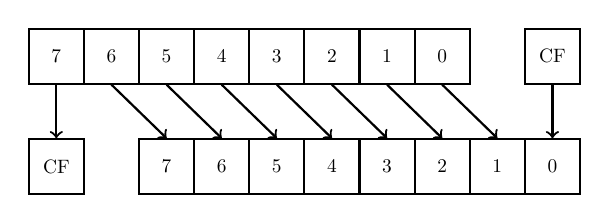
\begin{tikzpicture}[scale=0.7, every node/.style={scale=0.7}]
	\edef\bitsize{1cm}
	\tikzstyle{byte}=[draw,minimum size=\bitsize]	
	\tikzstyle{every path}=[thick]
	
	\node [draw,rectangle,minimum size=\bitsize] (a1) {7};
	\node [draw,rectangle,minimum size=\bitsize] (a2) [right of=a1] {6};
	\node [draw,rectangle,minimum size=\bitsize] (a3) [right of=a2] {5};
	\node [draw,rectangle,minimum size=\bitsize] (a4) [right of=a3] {4};
	\node [draw,rectangle,minimum size=\bitsize] (a5) [right of=a4] {3};
	\node [draw,rectangle,minimum size=\bitsize] (a6) [right of=a5] {2};
	\node [draw,rectangle,minimum size=\bitsize] (a7) [right of=a6] {1};
	\node [draw,rectangle,minimum size=\bitsize] (a8) [right of=a7] {0};
	\node (empty1) [right of=a8] {};
	\node [rectangle,draw,minimum size=\bitsize] (acf) [right of=empty1] {CF};
	
	\node (empty) [below of=a1] {};

	\node [rectangle,draw,minimum size=\bitsize] (bcf) [below of=empty] {CF};
	\node (empty2) [right of=bcf] {};
	\node [draw,rectangle,minimum size=\bitsize] (b1) [right of=empty2] {7};
	\node [draw,rectangle,minimum size=\bitsize] (b2) [right of=b1] {6};
	\node [draw,rectangle,minimum size=\bitsize] (b3) [right of=b2] {5};
	\node [draw,rectangle,minimum size=\bitsize] (b4) [right of=b3] {4};
	\node [draw,rectangle,minimum size=\bitsize] (b5) [right of=b4] {3};
	\node [draw,rectangle,minimum size=\bitsize] (b6) [right of=b5] {2};
	\node [draw,rectangle,minimum size=\bitsize] (b7) [right of=b6] {1};
	\node [draw,rectangle,minimum size=\bitsize] (b8) [right of=b7] {0};
	
	\draw [->] (a1.south) -- (bcf.north); % 7
	\draw [->] (a2.south) -- (b1.north); % 6
	\draw [->] (a3.south) -- (b2.north);
	\draw [->] (a4.south) -- (b3.north);
	\draw [->] (a5.south) -- (b4.north);
	\draw [->] (a6.south) -- (b5.north);
	\draw [->] (a7.south) -- (b6.north);
	\draw [->] (a8.south) -- (b7.north);
	\draw [->] (acf.south) -- (b8.north);

	\end{tikzpicture}
\end{center}

  \item[RCR] (M) \RU{вращать биты направо через флаг CF}\EN{rotate right via CF flag}:

\begin{center}
	\begin{tikzpicture}[scale=0.7, every node/.style={scale=0.7}]
	\edef\bitsize{1cm}
	\tikzstyle{byte}=[draw,minimum size=\bitsize]	
	\tikzstyle{every path}=[thick]

	\node [rectangle,draw,minimum size=\bitsize] (acf) {CF};
	\node (empty1) [right of=acf] {};
	
	\node [draw,rectangle,minimum size=\bitsize] (a1) [right of=empty1] {7};
	\node [draw,rectangle,minimum size=\bitsize] (a2) [right of=a1] {6};
	\node [draw,rectangle,minimum size=\bitsize] (a3) [right of=a2] {5};
	\node [draw,rectangle,minimum size=\bitsize] (a4) [right of=a3] {4};
	\node [draw,rectangle,minimum size=\bitsize] (a5) [right of=a4] {3};
	\node [draw,rectangle,minimum size=\bitsize] (a6) [right of=a5] {2};
	\node [draw,rectangle,minimum size=\bitsize] (a7) [right of=a6] {1};
	\node [draw,rectangle,minimum size=\bitsize] (a8) [right of=a7] {0};
	
	\node (empty) [below of=a1] {};

	\node [draw,rectangle,minimum size=\bitsize] (b1) [below of=empty] {7};
	\node [draw,rectangle,minimum size=\bitsize] (b2) [right of=b1] {6};
	\node [draw,rectangle,minimum size=\bitsize] (b3) [right of=b2] {5};
	\node [draw,rectangle,minimum size=\bitsize] (b4) [right of=b3] {4};
	\node [draw,rectangle,minimum size=\bitsize] (b5) [right of=b4] {3};
	\node [draw,rectangle,minimum size=\bitsize] (b6) [right of=b5] {2};
	\node [draw,rectangle,minimum size=\bitsize] (b7) [right of=b6] {1};
	\node [draw,rectangle,minimum size=\bitsize] (b8) [right of=b7] {0};
	
	\node (empty2) [right of=b7] {};
	
	\node [rectangle,draw,minimum size=\bitsize] (bcf) [right=of empty2] {CF};
	
	\draw [->] (acf.south) -- (b1.north);
	\draw [->] (a1.south) -- (b2.north);
	\draw [->] (a2.south) -- (b3.north);
	\draw [->] (a3.south) -- (b4.north);
	\draw [->] (a4.south) -- (b5.north);
	\draw [->] (a5.south) -- (b6.north);
	\draw [->] (a6.south) -- (b7.north);
	\draw [->] (a7.south) -- (b8.north);
	\draw [->] (a8.south) -- (bcf.north);

	\end{tikzpicture}
\end{center}


\myindex{x86!\Instructions!ROL}
\myindex{x86!\Instructions!ROR}
\label{ROL_ROR}
\item[ROL/ROR] (M) \RU{циклический сдвиг}\EN{cyclic shift}
  
ROL: \RU{вращать налево}\EN{rotate left}:

\begin{center}
	\begin{tikzpicture}[scale=0.7, every node/.style={scale=0.7}]
	\edef\bitsize{1cm}
	\tikzstyle{byte}=[draw,minimum size=\bitsize]	
	\tikzstyle{every path}=[thick]

	\node [draw,rectangle,minimum size=\bitsize] (a1) {7};
	\node [draw,rectangle,minimum size=\bitsize] (a2) [right of=a1] {6};
	\node [draw,rectangle,minimum size=\bitsize] (a3) [right of=a2] {5};
	\node [draw,rectangle,minimum size=\bitsize] (a4) [right of=a3] {4};
	\node [draw,rectangle,minimum size=\bitsize] (a5) [right of=a4] {3};
	\node [draw,rectangle,minimum size=\bitsize] (a6) [right of=a5] {2};
	\node [draw,rectangle,minimum size=\bitsize] (a7) [right of=a6] {1};
	\node [draw,rectangle,minimum size=\bitsize] (a8) [right of=a7] {0};

	\node (empty) [below of=a1] {};

	\node [draw,rectangle,minimum size=\bitsize] (b1) [below of=empty] {7};
	\node [draw,rectangle,minimum size=\bitsize] (b2) [right of=b1] {6};
	\node [draw,rectangle,minimum size=\bitsize] (b3) [right of=b2] {5};
	\node [draw,rectangle,minimum size=\bitsize] (b4) [right of=b3] {4};
	\node [draw,rectangle,minimum size=\bitsize] (b5) [right of=b4] {3};
	\node [draw,rectangle,minimum size=\bitsize] (b6) [right of=b5] {2};
	\node [draw,rectangle,minimum size=\bitsize] (b7) [right of=b6] {1};
	\node [draw,rectangle,minimum size=\bitsize] (b8) [right of=b7] {0};
	
	\node [shape=rectangle,draw,minimum size=\bitsize] (cf) [left=of b1] {CF};
	
	\draw [->] (a1.south) -- (b8.north);
	\draw [->] (a2.south) -- (b1.north);
	\draw [->] (a3.south) -- (b2.north);
	\draw [->] (a4.south) -- (b3.north);
	\draw [->] (a5.south) -- (b4.north);
	\draw [->] (a6.south) -- (b5.north);
	\draw [->] (a7.south) -- (b6.north);
	\draw [->] (a8.south) -- (b7.north);
	
	\draw [->] (a1.south) -- (cf.north);

	\end{tikzpicture}
\end{center}



ROR: \RU{вращать направо}\EN{rotate right}:

\begin{center}
	\begin{tikzpicture}[scale=0.7, every node/.style={scale=0.7}]
	\edef\bitsize{1cm}
	\tikzstyle{byte}=[draw,minimum size=\bitsize]	
	\tikzstyle{every path}=[thick]

	\node [draw,rectangle,minimum size=\bitsize] (a1) {7};
	\node [draw,rectangle,minimum size=\bitsize] (a2) [right of=a1] {6};
	\node [draw,rectangle,minimum size=\bitsize] (a3) [right of=a2] {5};
	\node [draw,rectangle,minimum size=\bitsize] (a4) [right of=a3] {4};
	\node [draw,rectangle,minimum size=\bitsize] (a5) [right of=a4] {3};
	\node [draw,rectangle,minimum size=\bitsize] (a6) [right of=a5] {2};
	\node [draw,rectangle,minimum size=\bitsize] (a7) [right of=a6] {1};
	\node [draw,rectangle,minimum size=\bitsize] (a8) [right of=a7] {0};

	\node (empty) [below of=a1] {};

	\node [draw,rectangle,minimum size=\bitsize] (b1) [below of=empty] {7};
	\node [draw,rectangle,minimum size=\bitsize] (b2) [right of=b1] {6};
	\node [draw,rectangle,minimum size=\bitsize] (b3) [right of=b2] {5};
	\node [draw,rectangle,minimum size=\bitsize] (b4) [right of=b3] {4};
	\node [draw,rectangle,minimum size=\bitsize] (b5) [right of=b4] {3};
	\node [draw,rectangle,minimum size=\bitsize] (b6) [right of=b5] {2};
	\node [draw,rectangle,minimum size=\bitsize] (b7) [right of=b6] {1};
	\node [draw,rectangle,minimum size=\bitsize] (b8) [right of=b7] {0};
	
	\node [shape=rectangle,draw,minimum size=\bitsize] (cf) [right=of b7] {CF};
	
	\draw [->] (a1.south) -- (b2.north);
	\draw [->] (a2.south) -- (b3.north);
	\draw [->] (a3.south) -- (b4.north);
	\draw [->] (a4.south) -- (b5.north);
	\draw [->] (a5.south) -- (b6.north);
	\draw [->] (a6.south) -- (b7.north);
	\draw [->] (a7.south) -- (b8.north);
	\draw [->] (a8.south) -- (b1.north);
	
	\draw [->] (a8.south) -- (cf.north);

	\end{tikzpicture}
\end{center}



\RU{Не смотря на то что многие \ac{CPU} имеют эти инструкции, в \CCpp нет соответствующих операций,
так что компиляторы с этих \ac{PL} обычно не генерируют код использующий эти инструкции}\EN{Despite the 
fact that almost all \ac{CPU}s have these instructions, there are no corresponding
operations in \CCpp, so the compilers of these \ac{PL}s usually do not generate these 
instructions}.

\RU{Чтобы программисту были доступны эти инструкции, в \ac{MSVC} есть псевдофункции}
\EN{For the programmer's convenience, at least \ac{MSVC} has the pseudofunctions} (compiler intrinsics)
\IT{\_rotl()} \AndENRU \IT{\_rotr()}\FNMSDNROTxURL{},
\RU{которые транслируются компилятором напрямую в эти инструкции}
\EN{which are translated by the compiler directly to these instructions}.


\myindex{x86!\Instructions!SAL}
  \item[SAL] \RU{Арифметический сдвиг влево}\EN{Arithmetic shift left}, \RU{синонимично}\EN{synonymous to} \TT{SHL}

\myindex{x86!\Instructions!SAR}
  \label{ins:SAR}
  \item[SAR] \RU{Арифметический сдвиг вправо}\EN{Arithmetic shift right}

\begin{center}
	\begin{tikzpicture}[scale=0.7, every node/.style={scale=0.7}]
	\edef\bitsize{1cm}
	\tikzstyle{byte}=[draw,minimum size=\bitsize]	
	\tikzstyle{every path}=[thick]

	\node [draw,rectangle,minimum size=\bitsize] (a1) {7};
	\node [draw,rectangle,minimum size=\bitsize] (a2) [right of=a1] {6};
	\node [draw,rectangle,minimum size=\bitsize] (a3) [right of=a2] {5};
	\node [draw,rectangle,minimum size=\bitsize] (a4) [right of=a3] {4};
	\node [draw,rectangle,minimum size=\bitsize] (a5) [right of=a4] {3};
	\node [draw,rectangle,minimum size=\bitsize] (a6) [right of=a5] {2};
	\node [draw,rectangle,minimum size=\bitsize] (a7) [right of=a6] {1};
	\node [draw,rectangle,minimum size=\bitsize] (a8) [right of=a7] {0};

	\node (empty) [below of=a1] {};

	\node [draw,rectangle,minimum size=\bitsize] (b1) [below of=empty] {7};
	\node [draw,rectangle,minimum size=\bitsize] (b2) [right of=b1] {6};
	\node [draw,rectangle,minimum size=\bitsize] (b3) [right of=b2] {5};
	\node [draw,rectangle,minimum size=\bitsize] (b4) [right of=b3] {4};
	\node [draw,rectangle,minimum size=\bitsize] (b5) [right of=b4] {3};
	\node [draw,rectangle,minimum size=\bitsize] (b6) [right of=b5] {2};
	\node [draw,rectangle,minimum size=\bitsize] (b7) [right of=b6] {1};
	\node [draw,rectangle,minimum size=\bitsize] (b8) [right of=b7] {0};
	
	\node [shape=rectangle,draw,minimum size=\bitsize] (cf) [right=of b7] {CF};
	
	\draw [->] (a1.south) -- (b1.north); %7
	\draw [->] (a1.south) -- (b2.north); %6

	\draw [->] (a2.south) -- (b3.north); %6
	\draw [->] (a3.south) -- (b4.north); %5
	\draw [->] (a4.south) -- (b5.north); %4
	\draw [->] (a5.south) -- (b6.north); %3
	\draw [->] (a6.south) -- (b7.north); %2
	\draw [->] (a7.south) -- (b8.north); %1
	
	\draw [->] (a8.south) -- (cf.north);

	\end{tikzpicture}
\end{center}

\RU{Таким образом, бит знака всегда остается на месте}
\EN{Hence, the sign bit always stays at the place of the} \ac{MSB}.


\myindex{x86!\Instructions!SETcc}
  \item[SETcc] op: \RU{загрузить 1 в op (только байт) если условие верно или 0 если наоборот}
  \EN{load 1 to operand (byte only) if the condition is true or zero otherwise}.
  \RU{Коды точно такие же, как и в инструкциях Jcc}\EN{The condition codes are the same as in the Jcc instructions} 
  (\myref{Jcc}).


\myindex{x86!\Instructions!STC}
\myindex{x86!\Flags!CF}
  \item[STC] (M) \RU{установить флаг CF}\EN{set CF flag}

\myindex{x86!\Instructions!STD}
\myindex{x86!\Flags!DF}
  \item[STD] (M) \RU{установить флаг DF}\EN{set DF flag}.
   \RU{Эта инструкция не генерируется компиляторами и вообще редкая.}
   \EN{This instruction is not generated by compilers and generally rare.}
   \RU{Например, она может быть найдена в файле}\EN{For example, it can be found in the} 
   \TT{ntoskrnl.exe} \RU{(ядро Windows) в написанных вручную функциях копирования 
   памяти}\EN{Windows kernel file, in the hand-written memory copy routines}.

\myindex{x86!\Instructions!STI}
\myindex{x86!\Flags!IF}
  \item[STI] (M) \RU{установить флаг IF}\EN{set IF flag}

\myindex{x86!\Instructions!SYSCALL}
  \item[SYSCALL] (AMD) \RU{вызов сисколла}\EN{call syscall} (\myref{syscalls})

\myindex{x86!\Instructions!SYSENTER}
  \item[SYSENTER] (Intel) \RU{вызов сисколла}\EN{call syscall} (\myref{syscalls})

\myindex{x86!\Instructions!UD2}
  \item[UD2] (M) \RU{неопределенная инструкция, вызывает исключение. Применяется для тестирования.}
  \EN{undefined instruction, raises exception. Used for testing.}

\myindex{x86!\Instructions!XCHG}
  \item[XCHG] (M) \RU{обменять местами значения в операндах}\EN{exchange the values in the operands}

\myindex{Borland Delphi}
\RU{Это редкая инструкция: компиляторы её не генерируют, потому что начиная с Pentium, XCHG с адресом в памяти в операнде
исполняется так, как если имеет префикс LOCK (см.\InSqBrackets{\MAbrash глава 19}).
Вероятно, в Intel так сделали для совместимости с синхронизирующими примитивами.
Таким образом, XCHG начиная с Pentium может быть медленной.
С другой стороны, XCHG была очень популярна у программистов на ассемблере.
Так что, если вы видите XCHG в коде, это может быть знаком, что код написан вручную.
Впрочем, по крайней мере компилятор Borland Delphi генерирует эту инструкцию.}
\EN{This instruction is rare: compilers don't generate it, because starting at Pentium, XCHG with address in memory in operand executes as if it has LOCK prefix (\InSqBrackets{\MAbrash chapter 19}).
Perhaps, Intel engineers did so for compatibility with synchronizing primitives.
Hence, XCHG starting at Pentium can be slow.
On the other hand, XCHG was very popular in assembly language programmers.
So if you see XCHG in code, it can be a sign that this piece of code is written manually.
However, at least Borland Delphi compiler generates this instruction.}



\end{description}

\subsubsection{\RU{Инструкции FPU}\EN{FPU instructions}}

\RU{Суффикс \TT{-R} в названии инструкции обычно означает, что операнды поменяны местами, суффикс \TT{-P} означает
что один элемент выталкивается из стека после исполнения инструкции, суффикс \TT{-PP} означает, что
выталкиваются два элемента}%
\EN{\TT{-R} suffix in the mnemonic usually implies that the operands are reversed,
\TT{-P} suffix implies that one element is popped
from the stack after the instruction's execution, \TT{-PP} suffix implies that two elements are popped}.

\TT{-P} \RU{инструкции часто бывают полезны, когда нам уже больше не нужно хранить значение в 
FPU-стеке после операции.}%
\EN{instructions are often useful when we do not need the value in the FPU stack to be 
present anymore after the operation.}

\begin{description}
\myindex{x86!\Instructions!FABS}
  \item[FABS] \RU{заменить значение в ST(0) на абсолютное значение ST(0)}\EN{replace value in ST(0) by absolute value in ST(0)}

\myindex{x86!\Instructions!FADD}
\myindex{x86!\Instructions!FADDP}
  \item[FADD] op: ST(0)=op+ST(0)
  \item[FADD] ST(0), ST(i): ST(0)=ST(0)+ST(i)
  \item[FADDP] ST(1)=ST(0)+ST(1);
  \RU{вытолкнуть один элемент из стека, таким образом, складываемые значения в стеке заменяются
  суммой}\EN{pop one element from the stack, i.e., the values in the stack are replaced by their sum}

 % + FADDP
\myindex{x86!\Instructions!FCHS}
  \item[FCHS] ST(0)=-ST(0)


\myindex{x86!\Instructions!FCOM}
\myindex{x86!\Instructions!FCOMP}
\myindex{x86!\Instructions!FCOMPP}
  \item[FCOM] \RU{сравнить}\EN{compare} ST(0) \RU{с}\EN{with} ST(1)
  \item[FCOM] op: \RU{сравнить}\EN{compare} ST(0) \RU{с}\EN{with} op
  \item[FCOMP] \RU{сравнить}\EN{compare} ST(0) \RU{с}\EN{with} ST(1); \RU{вытолкнуть один элемент из стека}
  \EN{pop one element from the stack}
  \item[FCOMPP] \RU{сравнить}\EN{compare} ST(0) \RU{с}\EN{with} ST(1); \RU{вытолкнуть два элемента из стека}
  \EN{pop two elements from the stack}

 % + FCOMP + FCOMPP
\myindex{x86!\Instructions!FDIVR}
\myindex{x86!\Instructions!FDIVRP}
  \item[FDIVR] op: ST(0)=op/ST(0)
  \item[FDIVR] ST(i), ST(j): ST(i)=ST(j)/ST(i)
  \item[FDIVRP] op: ST(0)=op/ST(0); \RU{вытолкнуть один элемент из стека}\EN{pop one element from the stack}
  \item[FDIVRP] ST(i), ST(j): ST(i)=ST(j)/ST(i); \RU{вытолкнуть один элемент из стека}\EN{pop one element from the stack}


 % + FDIVRP
\myindex{x86!\Instructions!FDIV}
\myindex{x86!\Instructions!FDIVP}
  \item[FDIV] op: ST(0)=ST(0)/op
  \item[FDIV] ST(i), ST(j): ST(i)=ST(i)/ST(j)
  \item[FDIVP] ST(1)=ST(0)/ST(1); \RU{вытолкнуть один элемент из стека, таким образом, 
  делимое и делитель в стеке заменяются частным}\EN{pop one element from the stack, i.e., 
  the dividend and divisor values in the stack are replaced by quotient}
 % + FDIVP
\myindex{x86!\Instructions!FILD}
  \item[FILD] op: \RU{сконвертировать целочисленный op и затолкнуть его в стек}
  \EN{convert integer and push it to the stack}.


\myindex{x86!\Instructions!FIST}
\myindex{x86!\Instructions!FISTP}
  \item[FIST] op: \RU{конвертировать}\EN{convert} ST(0) \RU{в целочисленное}\EN{to integer} op
  \item[FISTP] op: \RU{конвертировать}\EN{convert} ST(0) \RU{в целочисленное}\EN{to integer} op; 
  \RU{вытолкнуть один элемент из стека}\EN{pop one element from the stack}
 % + FISTP
\myindex{x86!\Instructions!FLD1}
  \item[FLD1] \RU{затолкнуть 1 в стек}\EN{push 1 to stack}


\myindex{x86!\Instructions!FLDCW}
  \item[FLDCW] op: \RU{загрузить}\EN{load} FPU control word (\myref{FPU_control_word}) \RU{из}\EN{from} 16-bit op.


\myindex{x86!\Instructions!FLDZ}
  \item[FLDZ] \RU{затолкнуть ноль в стек}\EN{push zero to stack}



\myindex{x86!\Instructions!FLD}
  \item[FLD] op: \RU{затолкнуть op в стек}\EN{push op to the stack}.

\myindex{x86!\Instructions!FMUL}
\myindex{x86!\Instructions!FMULP}
  \item[FMUL] op: ST(0)=ST(0)*op
  \item[FMUL] ST(i), ST(j): ST(i)=ST(i)*ST(j)
  \item[FMULP] op: ST(0)=ST(0)*op; \RU{вытолкнуть один элемент из стека}\EN{pop one element from the stack}
  \item[FMULP] ST(i), ST(j): ST(i)=ST(i)*ST(j); \RU{вытолкнуть один элемент из стека}\EN{pop one element from the stack}

 % + FMULP
\myindex{x86!\Instructions!FSINCOS}
  \item[FSINCOS]: tmp=ST(0); ST(1)=sin(tmp); ST(0)=cos(tmp)


\myindex{x86!\Instructions!FSQRT}
  \item[FSQRT]: $ST(0)=\sqrt{ST(0)}$


\myindex{x86!\Instructions!FSTCW}
\myindex{x86!\Instructions!FNSTCW}
  \item[FSTCW] op: \RU{записать}\EN{store} FPU control word (\myref{FPU_control_word}) \RU{в}\EN{into} 16-bit op
  \RU{после проверки ожидающих исключений}\EN{after checking for pending exceptions}.
  \item[FNSTCW] op: \RU{записать}\EN{store} FPU control word (\myref{FPU_control_word}) \RU{в}\EN{into} 16-bit op.

 % + FNSTCW
\myindex{x86!\Instructions!FSTSW}
\myindex{x86!\Instructions!FNSTSW}
  \item[FSTSW] op: \RU{записать}\EN{store} FPU status word (\myref{FPU_status_word}) \RU{в}\EN{into} 16-bit op
  \RU{после проверки ожидающих исключений}\EN{after checking for pending exceptions}.
  \item[FNSTSW] op: \RU{записать}\EN{store} FPU status word (\myref{FPU_status_word}) \RU{в}\EN{into} 16-bit op.

 % + FNSTSW
\myindex{x86!\Instructions!FST}
\myindex{x86!\Instructions!FSTP}
  \item[FST] op: \RU{копировать}\EN{copy} ST(0) \RU{в}\EN{to} op
  \item[FSTP] op: \RU{копировать}\EN{copy} ST(0) \RU{в}\EN{to} op; \RU{вытолкнуть один элемент из стека}
  \EN{pop one element from the stack}

\myindex{x86!\Instructions!FSUBR}
\myindex{x86!\Instructions!FSUBRP}
  \item[FSUBR] op: ST(0)=op-ST(0)
  \item[FSUBR] ST(0), ST(i): ST(0)=ST(i)-ST(0)
  \item[FSUBRP] ST(1)=ST(0)-ST(1);
  \RU{вытолкнуть один элемент из стека, таким образом, складываемые значения в стеке заменяются
  разностью}\EN{pop one element from the stack, i.e., the value in the stack is replaced by the difference}

 % + FSUBRP
\myindex{x86!\Instructions!FSUB}
\myindex{x86!\Instructions!FSUBP}
  \item[FSUB] op: ST(0)=ST(0)-op
  \item[FSUB] ST(0), ST(i): ST(0)=ST(0)-ST(i)
  \item[FSUBP] ST(1)=ST(1)-ST(0);
  \RU{вытолкнуть один элемент из стека, таким образом, складываемые значения в стеке заменяются
  разностью}\EN{pop one element from the stack, i.e., the value in the stack is replaced by the difference}

 % + FSUBP
\myindex{x86!\Instructions!FUCOM}
\myindex{x86!\Instructions!FUCOMP}
\myindex{x86!\Instructions!FUCOMPP}
  \item[FUCOM] ST(i): \RU{сравнить}\EN{compare} ST(0) \AndENRU ST(i)
  \item[FUCOM] \RU{сравнить}\EN{compare} ST(0) \AndENRU ST(1)
  \item[FUCOMP] \RU{сравнить}\EN{compare} ST(0) \AndENRU ST(1); \RU{вытолкнуть один элемент из стека}\EN{pop one element from stack}.
  \item[FUCOMPP] \RU{сравнить}\EN{compare} ST(0) \AndENRU ST(1); \RU{вытолкнуть два элемента из стека}\EN{pop two elements from stack}.
 
  \RU{Инструкция работает так же, как и FCOM, за тем исключением что исключение срабатывает только
  если один из операндов SNaN, но числа QNaN нормально обрабатываются}\EN{The instructions perform just like FCOM, but an exception is raised only if one of the operands is SNaN,
  while QNaN numbers are processed smoothly}.
 % + FUCOMP + FUCOMPP
\myindex{x86!\Instructions!FXCH}
  \item[FXCH] ST(i) \RU{обменять местами значения в ST(0) и ST(i)}\EN{exchange values in ST(0) and ST(i)}
  \item[FXCH] \RU{обменять местами значения в ST(0) и ST(1)}\EN{exchange values in ST(0) and ST(1)}


\end{description}

%\subsubsection{\RU{SIMD-инструкции}\EN{SIMD instructions}}

% TODO

%\begin{description}
%\input{appendix/x86/instructions/DIVSD}
%\input{appendix/x86/instructions/MOVDQA}
%\input{appendix/x86/instructions/MOVDQU}
%\input{appendix/x86/instructions/PADDD}
%\input{appendix/x86/instructions/PCMPEQB}
%\input{appendix/x86/instructions/PLMULHW}
%\input{appendix/x86/instructions/PLMULLD}
%\input{appendix/x86/instructions/PMOVMSKB}
%\input{appendix/x86/instructions/PXOR}
%\end{description}

% SHLD !
% SHRD !
% BSWAP !
% CMPXCHG
% XADD !
% CMPXCHG8B
% RDTSC !
% PAUSE!

% xsave
% fnclex, fnsave
% movsxd, movaps, wait, sfence, lfence, pushfq
% prefetchw
% REP RETN
% REP BSF
% movnti, movntdq, rdmsr, wrmsr
% ldmxcsr, stmxcsr, invlpg
% swapgs
% movq, movd
% mulsd
% POR
% IRETQ
% pslldq
% psrldq
% cqo, fxrstor, comisd, xrstor, wbinvd, movntq
% fprem
% addsb, subsd, frndint

% rare:
%\item[ENTER]
%\item[LES]
% LDS
% XLAT

\subsubsection{\RU{Инструкции с печатаемым ASCII-опкодом}\EN{Instructions having printable ASCII opcode}}

(\RU{В 32-битном режиме}\EN{In 32-bit mode}).

\label{printable_x86_opcodes}
\myindex{Shellcode}
\RU{Это может пригодиться для создания шеллкодов}\EN{These can be suitable for shellcode construction}.
\RU{См. также}\EN{See also}: \myref{subsec:EICAR}.

% FIXME: break table
\begin{center}
\begin{longtable}{ | l | l | l | }
\hline
\HeaderColor ASCII\RU{-символ}\EN{ character} & 
\HeaderColor \RU{шестнадцатеричный код}\EN{hexadecimal code} & 
\HeaderColor x86\RU{-инструкция}\EN{ instruction} \\
\hline
0	 &30	 &XOR \\
1	 &31	 &XOR \\
2	 &32	 &XOR \\
3	 &33	 &XOR \\
4	 &34	 &XOR \\
5	 &35	 &XOR \\
7	 &37	 &AAA \\
8	 &38	 &CMP \\
9	 &39	 &CMP \\
:	 &3a	 &CMP \\
;	 &3b	 &CMP \\
<	 &3c	 &CMP \\
=	 &3d	 &CMP \\
?	 &3f	 &AAS \\
@	 &40	 &INC \\
A	 &41	 &INC \\
B	 &42	 &INC \\
C	 &43	 &INC \\
D	 &44	 &INC \\
E	 &45	 &INC \\
F	 &46	 &INC \\
G	 &47	 &INC \\
H	 &48	 &DEC \\
I	 &49	 &DEC \\
J	 &4a	 &DEC \\
K	 &4b	 &DEC \\
L	 &4c	 &DEC \\
M	 &4d	 &DEC \\
N	 &4e	 &DEC \\
O	 &4f	 &DEC \\
P	 &50	 &PUSH \\
Q	 &51	 &PUSH \\
R	 &52	 &PUSH \\
S	 &53	 &PUSH \\
T	 &54	 &PUSH \\
U	 &55	 &PUSH \\
V	 &56	 &PUSH \\
W	 &57	 &PUSH \\
X	 &58	 &POP \\
Y	 &59	 &POP \\
Z	 &5a	 &POP \\
\lbrack{}	 &5b	 &POP \\
\textbackslash{}	 &5c	 &POP \\
\rbrack{}	 &5d	 &POP \\
\verb|^|	 &5e	 &POP \\
\_	 &5f	 &POP \\
\verb|`|	 &60	 &PUSHA \\
a	 &61	 &POPA \\
f	 &66	 &\RU{(в 32-битном режиме) переключиться на}\EN{(in 32-bit mode) switch to}\\
   & & \RU{16-битный размер операнда}\EN{16-bit operand size} \\
g	 &67	 &\RU{(в 32-битном режиме) переключиться на}\EN{in 32-bit mode) switch to}\\
   & & \RU{16-битный размер адреса}\EN{16-bit address size} \\
h	 &68	 &PUSH\\
i	 &69	 &IMUL\\
j	 &6a	 &PUSH\\
k	 &6b	 &IMUL\\
p	 &70	 &JO\\
q	 &71	 &JNO\\
r	 &72	 &JB\\
s	 &73	 &JAE\\
t	 &74	 &JE\\
u	 &75	 &JNE\\
v	 &76	 &JBE\\
w	 &77	 &JA\\
x	 &78	 &JS\\
y	 &79	 &JNS\\
z	 &7a	 &JP\\
\hline
\end{longtable}
\end{center}

\myindex{x86!\Instructions!AAA}
\myindex{x86!\Instructions!AAS}
\myindex{x86!\Instructions!CMP}
\myindex{x86!\Instructions!DEC}
\myindex{x86!\Instructions!IMUL}
\myindex{x86!\Instructions!INC}
\myindex{x86!\Instructions!JA}
\myindex{x86!\Instructions!JAE}
\myindex{x86!\Instructions!JB}
\myindex{x86!\Instructions!JBE}
\myindex{x86!\Instructions!JE}
\myindex{x86!\Instructions!JNE}
\myindex{x86!\Instructions!JNO}
\myindex{x86!\Instructions!JNS}
\myindex{x86!\Instructions!JO}
\myindex{x86!\Instructions!JP}
\myindex{x86!\Instructions!JS}
\myindex{x86!\Instructions!POP}
\myindex{x86!\Instructions!POPA}
\myindex{x86!\Instructions!PUSH}
\myindex{x86!\Instructions!PUSHA}
\myindex{x86!\Instructions!XOR}

\RU{В итоге}\EN{In summary}:
AAA, AAS, CMP, DEC, IMUL, INC, JA, JAE, JB, JBE, JE, JNE, JNO, JNS, JO, JP, JS, POP, POPA, PUSH, PUSHA, 
XOR.

